% =====================================================================
%  Лабораторийн ажил №1 — Цаг агаарын мэдээллийн системийн
%  өгөгдлийн сангийн дизайн (Relational + NoSQL)
%  Хөрвүүлэгч: XeLaTeX  (Overleaf: Menu -> Compiler -> XeLaTeX)
% =====================================================================
\documentclass[12pt,a4paper]{article}

% ---------- Хуудасны хэмжээ, мөр хоорондын зай ----------
\usepackage[a4paper,left=3cm,right=1.5cm,top=2cm,bottom=2cm,footskip=1cm]{geometry}
\usepackage{setspace}
\onehalfspacing
\setlength{\parindent}{1.25cm}
\setlength{\parskip}{3pt}
\emergencystretch=3em

% ---------- Фонт: Times New Roman (байхгүй бол Liberation Serif) ----------
\usepackage{fontspec}
\IfFontExistsTF{Times New Roman}{%
  \setmainfont{Times New Roman}%
}{%
  \setmainfont{LiberationSerif}[
    Path=fonts/, Extension=.ttf,
    UprightFont=*-Regular, BoldFont=*-Bold,
    ItalicFont=*-Italic, BoldItalicFont=*-BoldItalic]%
}
\setmonofont{DejaVuSansMono}[Path=fonts/, Extension=.ttf, Scale=0.85]

% ---------- Багцууд ----------
\usepackage{graphicx}
\usepackage{xcolor}
\usepackage{array}
\usepackage{longtable}
\usepackage{booktabs}
\usepackage{caption}
\usepackage{enumitem}
\usepackage{fancyvrb}
\usepackage{titlesec}
\usepackage{tocloft}
\usepackage{pdflscape}
\usepackage{tikz}
\usetikzlibrary{positioning,arrows.meta,shapes.geometric}
\usepackage[hidelinks]{hyperref}

% ---------- Монгол нэршил ----------
\renewcommand{\contentsname}{ГАРЧИГ}
\renewcommand{\listfigurename}{ЗУРГИЙН ЖАГСААЛТ}
\renewcommand{\listtablename}{ХҮСНЭГТИЙН ЖАГСААЛТ}
\renewcommand{\figurename}{Зураг}
\renewcommand{\tablename}{Хүснэгт}
\captionsetup{labelsep=period,font=small,labelfont=bf,skip=6pt}
\captionsetup[table]{position=top}

% Гарчиг, жагсаалтын толгой — голлуулсан, 14pt тод
\renewcommand{\cfttoctitlefont}{\hfill\fontsize{14}{17}\selectfont\bfseries}
\renewcommand{\cftaftertoctitle}{\hfill\mbox{}}
\renewcommand{\cftloftitlefont}{\hfill\fontsize{14}{17}\selectfont\bfseries}
\renewcommand{\cftafterloftitle}{\hfill\mbox{}}
\renewcommand{\cftlottitlefont}{\hfill\fontsize{14}{17}\selectfont\bfseries}
\renewcommand{\cftafterlottitle}{\hfill\mbox{}}
\renewcommand{\cftsecleader}{\cftdotfill{\cftdotsep}}
\renewcommand{\cftfigpresnum}{Зураг~}
\renewcommand{\cfttabpresnum}{Хүснэгт~}
\setlength{\cftfignumwidth}{5.5em}
\setlength{\cfttabnumwidth}{6.5em}

% Бүлгийн гарчгийн хэмжээ (14pt / 12pt)
\titleformat{\section}{\fontsize{14}{17}\selectfont\bfseries}{\thesection.}{0.5em}{}
\titleformat{\subsection}{\fontsize{12}{15}\selectfont\bfseries}{\thesubsection}{0.5em}{}
\titlespacing*{\section}{0pt}{12pt}{6pt}
\titlespacing*{\subsection}{0pt}{10pt}{4pt}

\setlist{itemsep=1pt,topsep=3pt}
\newcolumntype{L}[1]{>{\raggedright\arraybackslash}p{#1}}
\newcolumntype{C}[1]{>{\centering\arraybackslash}p{#1}}
\newcommand{\pk}[1]{\textbf{#1}}

% Хуудасны дугаар: доод хэсгийн голд, араб тоогоор (plain стиль)
\pagestyle{plain}

\begin{document}

% =====================================================================
%  НҮҮР ХУУДАС (дугаарлалтад орохгүй)
% =====================================================================
\begin{titlepage}
\centering
\singlespacing
{\fontsize{13}{16}\selectfont\bfseries ШИНЖЛЭХ УХААН ТЕХНОЛОГИЙН ИХ СУРГУУЛЬ\par}
\vspace{0.5cm}
{\fontsize{12}{15}\selectfont\bfseries МЭДЭЭЛЭЛ ХОЛБООНЫ ТЕХНОЛОГИЙН СУРГУУЛЬ\par}

\vspace{1.8cm}

\includegraphics[height=5.2cm]{images/logo.png}\par

\vspace{2.2cm}
{\fontsize{20}{26}\selectfont\bfseries ЛАБОРАТОРИЙН АЖЛЫН\par}
\vspace{0.6cm}
{\fontsize{20}{26}\selectfont\bfseries ТАЙЛАН\par}

\vspace{1.4cm}
{\bfseries Өгөгдлийн сангийн удирдлага (F.ITM237)\par}
\vspace{0.5cm}
{\bfseries Сэдэв: Лабораторийн ажил 1\par}
\vspace{0.3cm}
{\itshape Цаг агаарын мэдээллийн системийн өгөгдлийн сангийн дизайн\par}

\vspace{2.2cm}
\begin{flushleft}
\begin{tabular}{@{}p{10.5cm}l@{}}
\textbf{Гүйцэтгэсэн оюутан:} Ц.Номинжин /B241940137/ & /\,\makebox[4.3cm]{\dotfill}\,/ \\[0.9cm]
\textbf{Шалгасан багш:} С.Өлзийбаяр /F.IT14/ & /\,\makebox[4.3cm]{\dotfill}\,/ \\
\end{tabular}
\end{flushleft}

\vfill
Улаанбаатар 2026 он
\end{titlepage}

% Нүүр хуудсыг дугаарлалтад оруулахгүй: дараагийн хуудаснаас 1-ээс эхэлнэ
\pagenumbering{arabic}
\setcounter{page}{1}

% =====================================================================
%  ГАРЧИГ, ЖАГСААЛТУУД
% =====================================================================
\tableofcontents
\clearpage
\addcontentsline{toc}{section}{Зургийн жагсаалт}
\listoffigures
\vspace{1cm}
\addcontentsline{toc}{section}{Хүснэгтийн жагсаалт}
\listoftables
\clearpage

% =====================================================================
\section{Системийн тодорхойлолт}
% =====================================================================
\textbf{Сэдэв:} «ЦагАгаар» — Монгол орны аймаг, сумдын цаг уурын станцуудаас
хэмжилт цуглуулж, урьдчилсан мэдээ болон аюултай үзэгдлийн сэрэмжлүүлгийг
иргэдэд хүргэх үндэсний цаг агаарын мэдээллийн систем.

\subsection{Системийн зорилго}
\begin{itemize}
  \item Автомат болон гар ажиллагаатай станцуудын мэдрэгчээс минут тутмын хэмжилтийг найдвартай цуглуулж хадгалах.
  \item Түүхий хэмжилтийг шалгаж, цаг тутмын баталгаажсан ажиглалт (Observation) болгон нэгтгэх.
  \item Синоптикчид байршил бүрээр урьдчилсан мэдээ гаргах.
  \item Шуурга, зуд, үер зэрэг аюултай үзэгдлийн сэрэмжлүүлгийг хамрах нутгийн иргэдэд SMS, и-мэйл, push-ээр шуурхай хүргэх.
  \item Станцын тоног төхөөрөмжийн засвар үйлчилгээг бүртгэж, мэдрэгчийн тасалдлыг хянах.
\end{itemize}

\subsection{Үндсэн хэрэглэгчид (roles)}
\begin{longtable}{L{3.6cm}L{4.4cm}L{7.0cm}}
\caption{Системийн хэрэглэгчид ба эрх}\label{tab:roles}\\
\toprule
\textbf{Role} & \textbf{Хэн бэ} & \textbf{Үндсэн эрх}\\
\midrule
\endfirsthead
\toprule
\textbf{Role} & \textbf{Хэн бэ} & \textbf{Үндсэн эрх}\\
\midrule
\endhead
Иргэн (Citizen) & Малчин, жолооч, аялагч г.м. олон нийт & Мэдээ харах, байршил захиалах, ажигласан үзэгдлээ мэдээлэх, сэтгэгдэл бичих\\
Синоптикч (Forecaster) & Цаг уурын шинжээч ажилтан & Урьдчилсан мэдээ болон сэрэмжлүүлэг гаргах\\
Станцын техникч (Technician) & Станц хариуцсан инженер & Станц, мэдрэгч бүртгэх, засвар үйлчилгээ хийх\\
Админ (Admin) & Системийн администратор & Хэрэглэгч, байршил, эрхийн удирдлага\\
\bottomrule
\end{longtable}

\subsection{Хадгалах өгөгдлийн төрөл}
\begin{itemize}
  \item \textbf{Лавлах өгөгдөл:} хэрэглэгч, ажилтан, байршил (аймаг/сум, координат), станц, мэдрэгч.
  \item \textbf{Бизнесийн гүйлгээний өгөгдөл:} цаг тутмын ажиглалт, урьдчилсан мэдээ, сэрэмжлүүлэг, захиалга, засвар үйлчилгээ.
  \item \textbf{Их хэмжээний / хувьсах бүтэцтэй өгөгдөл:} мэдрэгчийн минут тутмын түүхий хэмжилт, хэрэглэгчийн үйлдлийн лог, мэдэгдэл илгээлтийн түүх, иргэдийн мэдээлэл (зураг, сэтгэгдэл, like).
\end{itemize}

\subsection{Бизнес процессууд}
\begin{enumerate}
  \item \textbf{Хэмжилт цуглуулах:} мэдрэгч минут тутам утга илгээнэ $\rightarrow$ NoSQL \texttt{sensor\_readings}-д бичигдэнэ.
  \item \textbf{Ажиглалт нэгтгэх:} цаг бүр түүхий утгыг шалгаж, станц бүрийн баталгаажсан \texttt{Observation} мөр үүснэ.
  \item \textbf{Урьдчилсан мэдээ гаргах:} синоптикч ажиглалтад тулгуурлан байршил бүрт \texttt{Forecast} гаргана.
  \item \textbf{Сэрэмжлүүлэг зарлах:} синоптикч \texttt{WeatherAlert} үүсгэж, хамрах байршлуудыг (\texttt{AlertArea}) сонгоно.
  \item \textbf{Мэдэгдэл хүргэх:} тухайн байршлыг захиалсан (\texttt{Subscription}) иргэдэд сэрэмжлүүлэг илгээгдэж, үр дүн нь \texttt{notification\_logs}-д хадгалагдана.
  \item \textbf{Иргэний мэдээлэл:} иргэн ажигласан үзэгдлээ зурагтай мэдээлж (\texttt{community\_reports}), бусад нь сэтгэгдэл, like үлдээнэ.
  \item \textbf{Засвар үйлчилгээ:} техникч станцад хийсэн засвар, калибровкийг \texttt{Maintenance}-д бүртгэнэ.
\end{enumerate}

Өгөгдлийн үндсэн урсгалыг \ref{fig:flow}-р зурагт харуулав.

\begin{figure}[htbp]
\centering
\begin{tikzpicture}[
  node distance=0.55cm and 1.5cm,
  sql/.style={draw=blue!60!black,fill=blue!8,rounded corners=2pt,minimum width=3.0cm,minimum height=1.1cm,align=center,font=\small},
  nos/.style={draw=orange!70!black,fill=orange!12,double,rounded corners=2pt,minimum width=2.9cm,minimum height=1cm,align=center,font=\small},
  ar/.style={-{Stealth[length=2.2mm]},thick,gray!70!black},
  lb/.style={font=\scriptsize,fill=white,inner sep=1pt}]
  \node[sql] (sen) {Sensor\\(SQL)};
  \node[nos,right=of sen] (rd) {SensorReadings\\(NoSQL)};
  \node[sql,right=of rd] (obs) {Observation\\(SQL)};
  \node[sql,below=1.3cm of obs] (fc) {Forecast\\(SQL)};
  \node[sql,left=of fc] (al) {WeatherAlert +\\AlertArea (SQL)};
  \node[nos,left=of al] (nl) {NotificationLog\\(NoSQL)};
  \draw[ar] (sen) -- node[lb,above=2pt]{минут бүр} (rd);
  \draw[ar] (rd) -- node[lb,above=2pt]{цаг бүр} (obs);
  \draw[ar] (obs) -- node[lb,right=2pt]{синоптикч} (fc);
  \draw[ar] (obs.south west) -- (al.north east);
  \draw[ar] (al) -- node[lb,above=2pt]{Subscription} (nl);
\end{tikzpicture}
\caption{Өгөгдлийн урсгал: мэдрэгчээс сэрэмжлүүлэг хүртэл}\label{fig:flow}
\end{figure}

% =====================================================================
\section{Entity-ийн жагсаалт ба тайлбар}
% =====================================================================
Загвар нийт \textbf{15 entity}-тэй: \textbf{11 relational} (R1--R11) ба
\textbf{4 NoSQL} (N1--N4). Primary key-г \textbf{тод} бичвэрээр,
гадаад түлхүүрийг (FK) \textit{налуу} бичвэрээр тэмдэглэв. FK нь conceptual
ERD дээр атрибут биш, холбоосоор илэрнэ.

\subsection{Relational entity-үүд}
{\small
\setlength{\tabcolsep}{4pt}
\begin{longtable}{C{0.7cm}L{2.8cm}L{2.7cm}L{4.9cm}L{3.8cm}}
\caption{Relational entity-үүд, атрибут ба PK}\label{tab:rel}\\
\toprule
\textbf{№} & \textbf{Entity} & \textbf{PK} & \textbf{Атрибутууд} & \textbf{Тайлбар}\\
\midrule
\endfirsthead
\toprule
\textbf{№} & \textbf{Entity} & \textbf{PK} & \textbf{Атрибутууд} & \textbf{Тайлбар}\\
\midrule
\endhead
\bottomrule
\endfoot
R1 & \textbf{User} (Хэрэглэгч) & \pk{user\_id} & full\_name, email, phone, password\_hash, role, created\_at & Системд бүртгэлтэй бүх хүн (иргэн, ажилтан, админ)\\
R2 & \textbf{Staff} (Ажилтан) & \pk{staff\_id} & \textit{user\_id}, position, department, license\_no, hired\_date & Синоптикч, техникчийн албан мэдээлэл; User-тэй 1:1\\
R3 & \textbf{Location} (Байршил) & \pk{location\_id} & name, aimag, soum, latitude, longitude, elevation\_m & Урьдчилсан мэдээ, сэрэмжлүүлэг хамаарах газарзүйн нэгж\\
R4 & \textbf{WeatherStation} (Цаг уурын станц) & \pk{station\_id} & \textit{location\_id}, station\_code, name, station\_type (auto/manual), install\_date, status & Хэмжилт хийдэг физик станц\\
R5 & \textbf{Sensor} (Мэдрэгч) & \pk{sensor\_id} & \textit{station\_id}, sensor\_type, model, unit, calibration\_date, status & Температур, чийгшил, даралт, салхи, тунадасны мэдрэгч\\
R6 & \textbf{Observation} (Ажиглалт) & \pk{observation\_\allowbreak id} & \textit{station\_id}, observed\_at, temperature\_c, humidity\_pct, pressure\_hpa, wind\_speed\_ms, wind\_dir\_deg, precipitation\_mm, quality\_flag & Цаг тутмын шалгагдсан, баталгаажсан хэмжилт\\
R7 & \textbf{Forecast} (Урьдчилсан мэдээ) & \pk{forecast\_id} & \textit{location\_id}, \textit{staff\_id}, issued\_at, valid\_from, valid\_to, temp\_min\_c, temp\_max\_c, condition, precip\_prob\_pct, wind\_speed\_ms & Байршил бүрийн хугацаатай урьдчилан мэдээ\\
R8 & \textbf{WeatherAlert} (Сэрэмжлүүлэг) & \pk{alert\_id} & \textit{staff\_id}, alert\_type, severity, title, description, start\_time, end\_time & Аюултай үзэгдлийн албан сэрэмжлүүлэг\\
R9 & \textbf{AlertArea} (Хамрах нутаг) & \pk{alert\_id + location\_id} & risk\_level, added\_at & Association entity: WeatherAlert M:N Location\\
R10 & \textbf{Subscription} (Захиалга) & \pk{subscription\_\allowbreak id} & \textit{user\_id}, \textit{location\_id}, channel (SMS/email/push), min\_severity, is\_active, created\_at & Association entity: User M:N Location\\
R11 & \textbf{Maintenance} (Засвар үйлчилгээ) & \pk{maintenance\_\allowbreak id} & \textit{station\_id}, \textit{staff\_id}, performed\_at, maint\_type, description, cost\_mnt & Станцын засвар, калибровкийн түүх\\
\end{longtable}
}

\subsection{NoSQL entity-үүд (document collection)}
{\small
\setlength{\tabcolsep}{4pt}
\begin{longtable}{C{0.7cm}L{3.0cm}L{1.1cm}L{6.0cm}L{4.1cm}}
\caption{NoSQL collection-ууд ба бүтэц}\label{tab:nosql}\\
\toprule
\textbf{№} & \textbf{Collection} & \textbf{PK} & \textbf{Бүтэц (embedded / array)} & \textbf{Тайлбар}\\
\midrule
\endfirsthead
\toprule
\textbf{№} & \textbf{Collection} & \textbf{PK} & \textbf{Бүтэц (embedded / array)} & \textbf{Тайлбар}\\
\midrule
\endhead
\bottomrule
\endfoot
N1 & \textbf{SensorReadings} & \pk{\_id} & sensor\_id, station\_id, hour\_bucket, readings: [\{ts, value, raw\_signal\} … 60 ширхэг], stats: \{min, max, avg\} & Минут тутмын түүхий хэмжилт, нэг цагийн багц (bucket)\\
N2 & \textbf{UserActivityLog} & \pk{\_id} & user\_id, date, device: \{os, app\_version\}, events: [\{ts, action, location\_id, meta\}] & Хэрэглэгчийн хайлт, харсан байршил, товшилт\\
N3 & \textbf{NotificationLog} & \pk{\_id} & alert\_id, sent\_at, summary: \{total, delivered, failed\}, deliveries: [\{user\_id, channel, status, delivered\_at, error\}] & Сэрэмжлүүлэг бүрийн илгээлтийн түүх\\
N4 & \textbf{CommunityReport} & \pk{\_id} & user\_id, location\_id, created\_at, phenomenon, text, photos: [url], geo: \{lat, lng\}, comments: [\{user\_id, text, ts\}], likes: [user\_id] & Иргэдийн ажигласан үзэгдлийн мэдээлэл\\
\end{longtable}
}

\subsection{Холбоосууд (relationship)}
{\small
\begin{longtable}{L{3.7cm}L{2.5cm}L{3.3cm}C{1.3cm}L{3.5cm}}
\caption{Холбоосууд, cardinality ба participation}\label{tab:rels}\\
\toprule
\textbf{Relationship} & \textbf{Entity A} & \textbf{Entity B} & \textbf{Card.} & \textbf{Participation}\\
\midrule
\endfirsthead
\toprule
\textbf{Relationship} & \textbf{Entity A} & \textbf{Entity B} & \textbf{Card.} & \textbf{Participation}\\
\midrule
\endhead
\bottomrule
\endfoot
АЖИЛТАН\_БАЙХ & User & Staff & 1 : 1 & User — хэсэгчилсэн, Staff — бүрэн\\
БАЙРЛАХ & Location & WeatherStation & 1 : N & Station — бүрэн\\
СУУРИЛУУЛСАН & WeatherStation & Sensor & 1 : N & Sensor — бүрэн\\
БҮРТГЭХ & WeatherStation & Observation & 1 : N & Observation — бүрэн\\
ХАМААРАХ & Location & Forecast & 1 : N & Forecast — бүрэн\\
ГАРГАХ & Staff & Forecast & 1 : N & Forecast — бүрэн\\
ЗАРЛАХ & Staff & WeatherAlert & 1 : N & Alert — бүрэн\\
ХАМРАХ (AlertArea) & WeatherAlert & Location & M : N & Alert — бүрэн, Location — хэсэгчилсэн\\
ЗАХИАЛАХ (Subscription) & User & Location & M : N & Хоёр тал хэсэгчилсэн\\
ҮЙЛЧЛҮҮЛЭХ & WeatherStation & Maintenance & 1 : N & Maintenance — бүрэн\\
ГҮЙЦЭТГЭХ & Staff & Maintenance & 1 : N & Maintenance — бүрэн\\
ХЭМЖИХ & Sensor & SensorReadings (NoSQL) & 1 : N & Readings — бүрэн\\
ҮЙЛДЭЛ\_ХИЙХ & User & UserActivityLog (NoSQL) & 1 : N & Log — бүрэн\\
ИЛГЭЭХ & WeatherAlert & NotificationLog (NoSQL) & 1 : N & Log — бүрэн\\
МЭДЭЭЛЭХ & User & CommunityReport (NoSQL) & 1 : N & Report — бүрэн\\
ТУХАЙН & Location & CommunityReport (NoSQL) & 1 : N & Report — бүрэн\\
\end{longtable}
}

% =====================================================================
\section{ERD (Chen diagram)}
% =====================================================================
\ref{fig:erdfull}-р зурагт бүх entity, атрибут, холбоосыг нэг дор харуулсан бүрэн
Chen ERD-г үзүүлэв. Үүнийг уншихад хялбар болгох үүднээс дараах 3 зурагт хуваав:
\ref{fig:erd}-р зурагт 15 entity, 16 холбоосыг зөвхөн entity, relationship,
cardinality ба participation-ийн түвшинд харуулсан ерөнхий Chen ERD;
\ref{fig:relattr}-р зурагт relational entity-үүдийн атрибутууд;
\ref{fig:nosqlattr}-р зурагт NoSQL collection-уудын атрибут, embedded document
ба array бүтэц. Цэнхэр өнгө нь relational, улбар шар давхар хүрээтэй нь NoSQL
хэсгийг илэрхийлнэ.

\noindent\textbf{Тэмдэглэгээний тайлбар:}
\begin{itemize}
  \item \textbf{Тэгш өнцөгт} — entity; цэнхэр дүүргэлттэй нь relational, улбар шар \textbf{давхар хүрээтэй} нь NoSQL collection (weak / embedded entity ба «NoSQL» гэсэн шошготой).
  \item \textbf{Ромб} — relationship, нэр нь монгол үйл үгээр; NoSQL entity-тэй холбох identifying relationship нь давхар ромб.
  \item \textbf{Тод хүрээтэй том ромб} (ХАМРАХ / AlertArea, ЗАХИАЛАХ / Subscription) — M:N холбоосыг задлах association entity, өөрийн атрибуттай.
  \item \textbf{Зууван} — атрибут; \textbf{доогуур зураастай} нь PK; \textbf{давхар зууван} (\texttt{readings[]}, \texttt{likes[]} г.м.) нь array / олон утгат атрибут; дэд зуувантай атрибут (\texttt{geo}, \texttt{stats}, \texttt{device}) нь embedded document.
  \item \textbf{Давхар шугам} — total participation (заавал оролцоно), \textbf{ганц шугам} — partial participation.
  \item \textbf{Улаан 1 / N / M} — cardinality. Жишээ: нэг Location-д олон WeatherStation байрлах (1:N), станц бүр заавал нэг байршилтай (total).
  \item FK багануудыг диаграм дээр зориудаар зураагүй — conceptual түвшинд холбоос нь ромбоор илэрдэг.
\end{itemize}

\begin{landscape}
\begin{figure}[p]
\centering
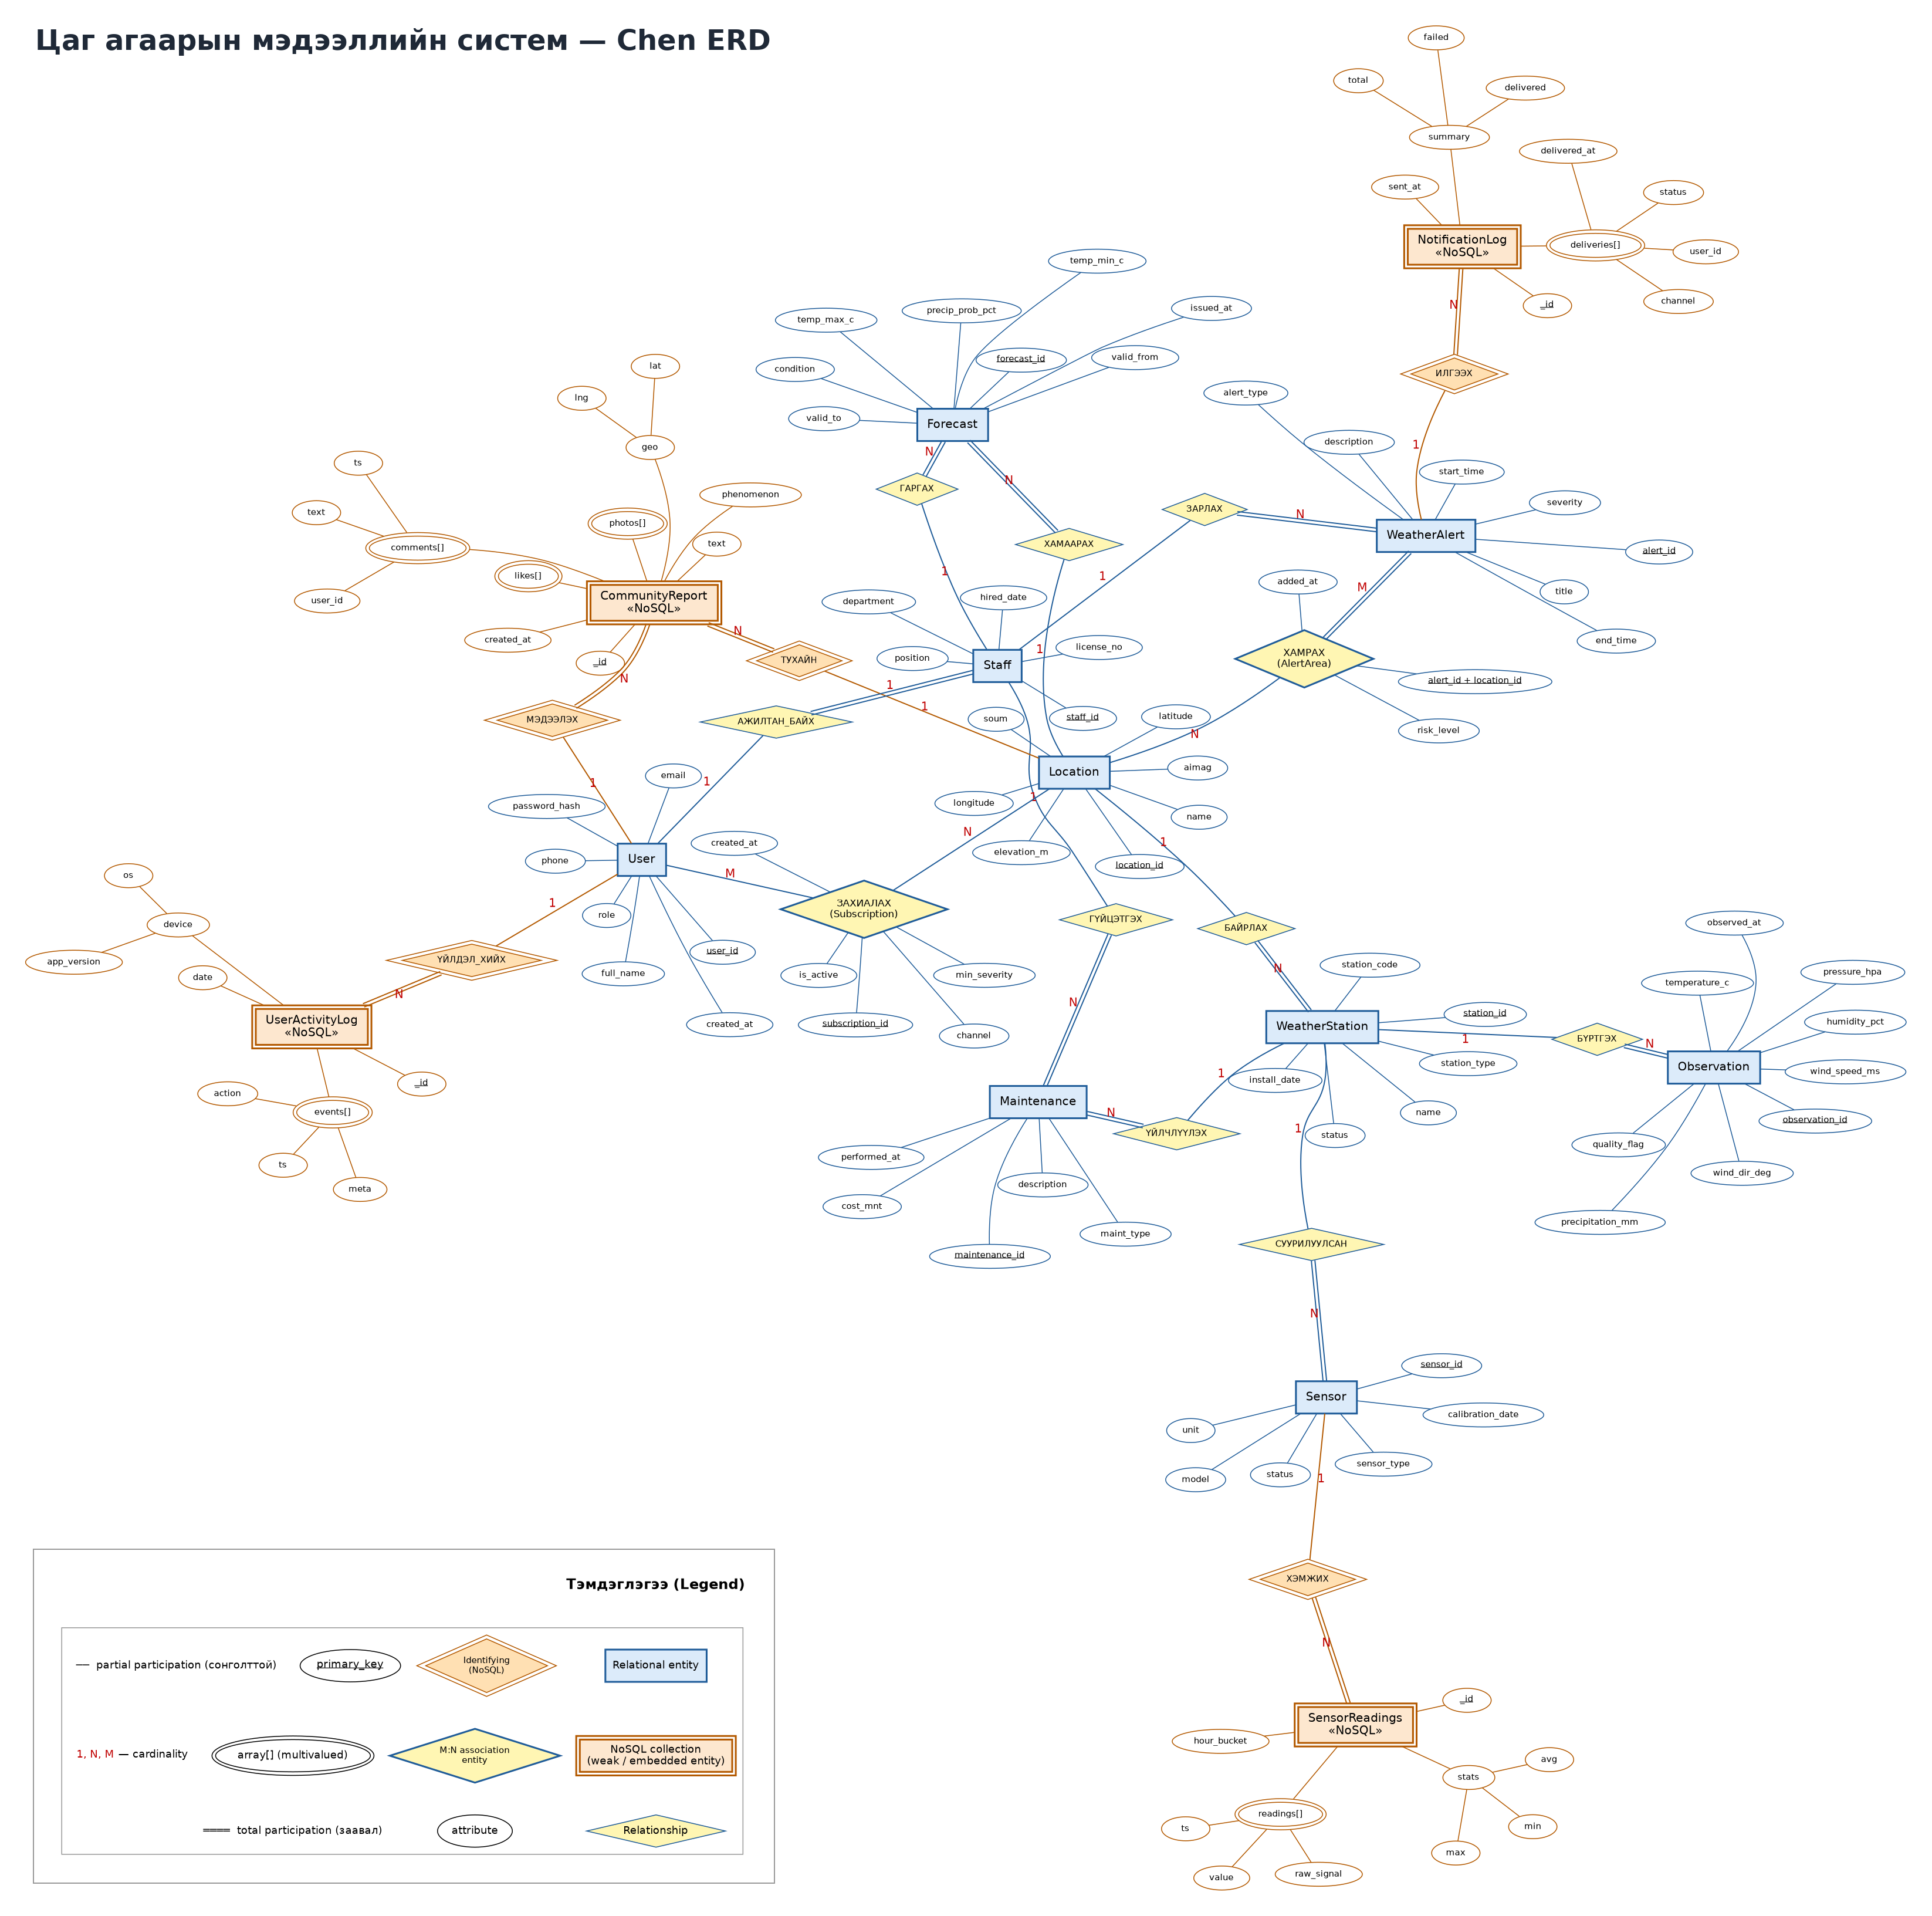
\includegraphics[width=\linewidth,height=0.93\textheight,keepaspectratio]{images/erd_full.png}
\caption{Бүрэн Chen ERD: entity, атрибут, холбоос ба cardinality}\label{fig:erdfull}
\end{figure}
\begin{figure}[p]
\centering
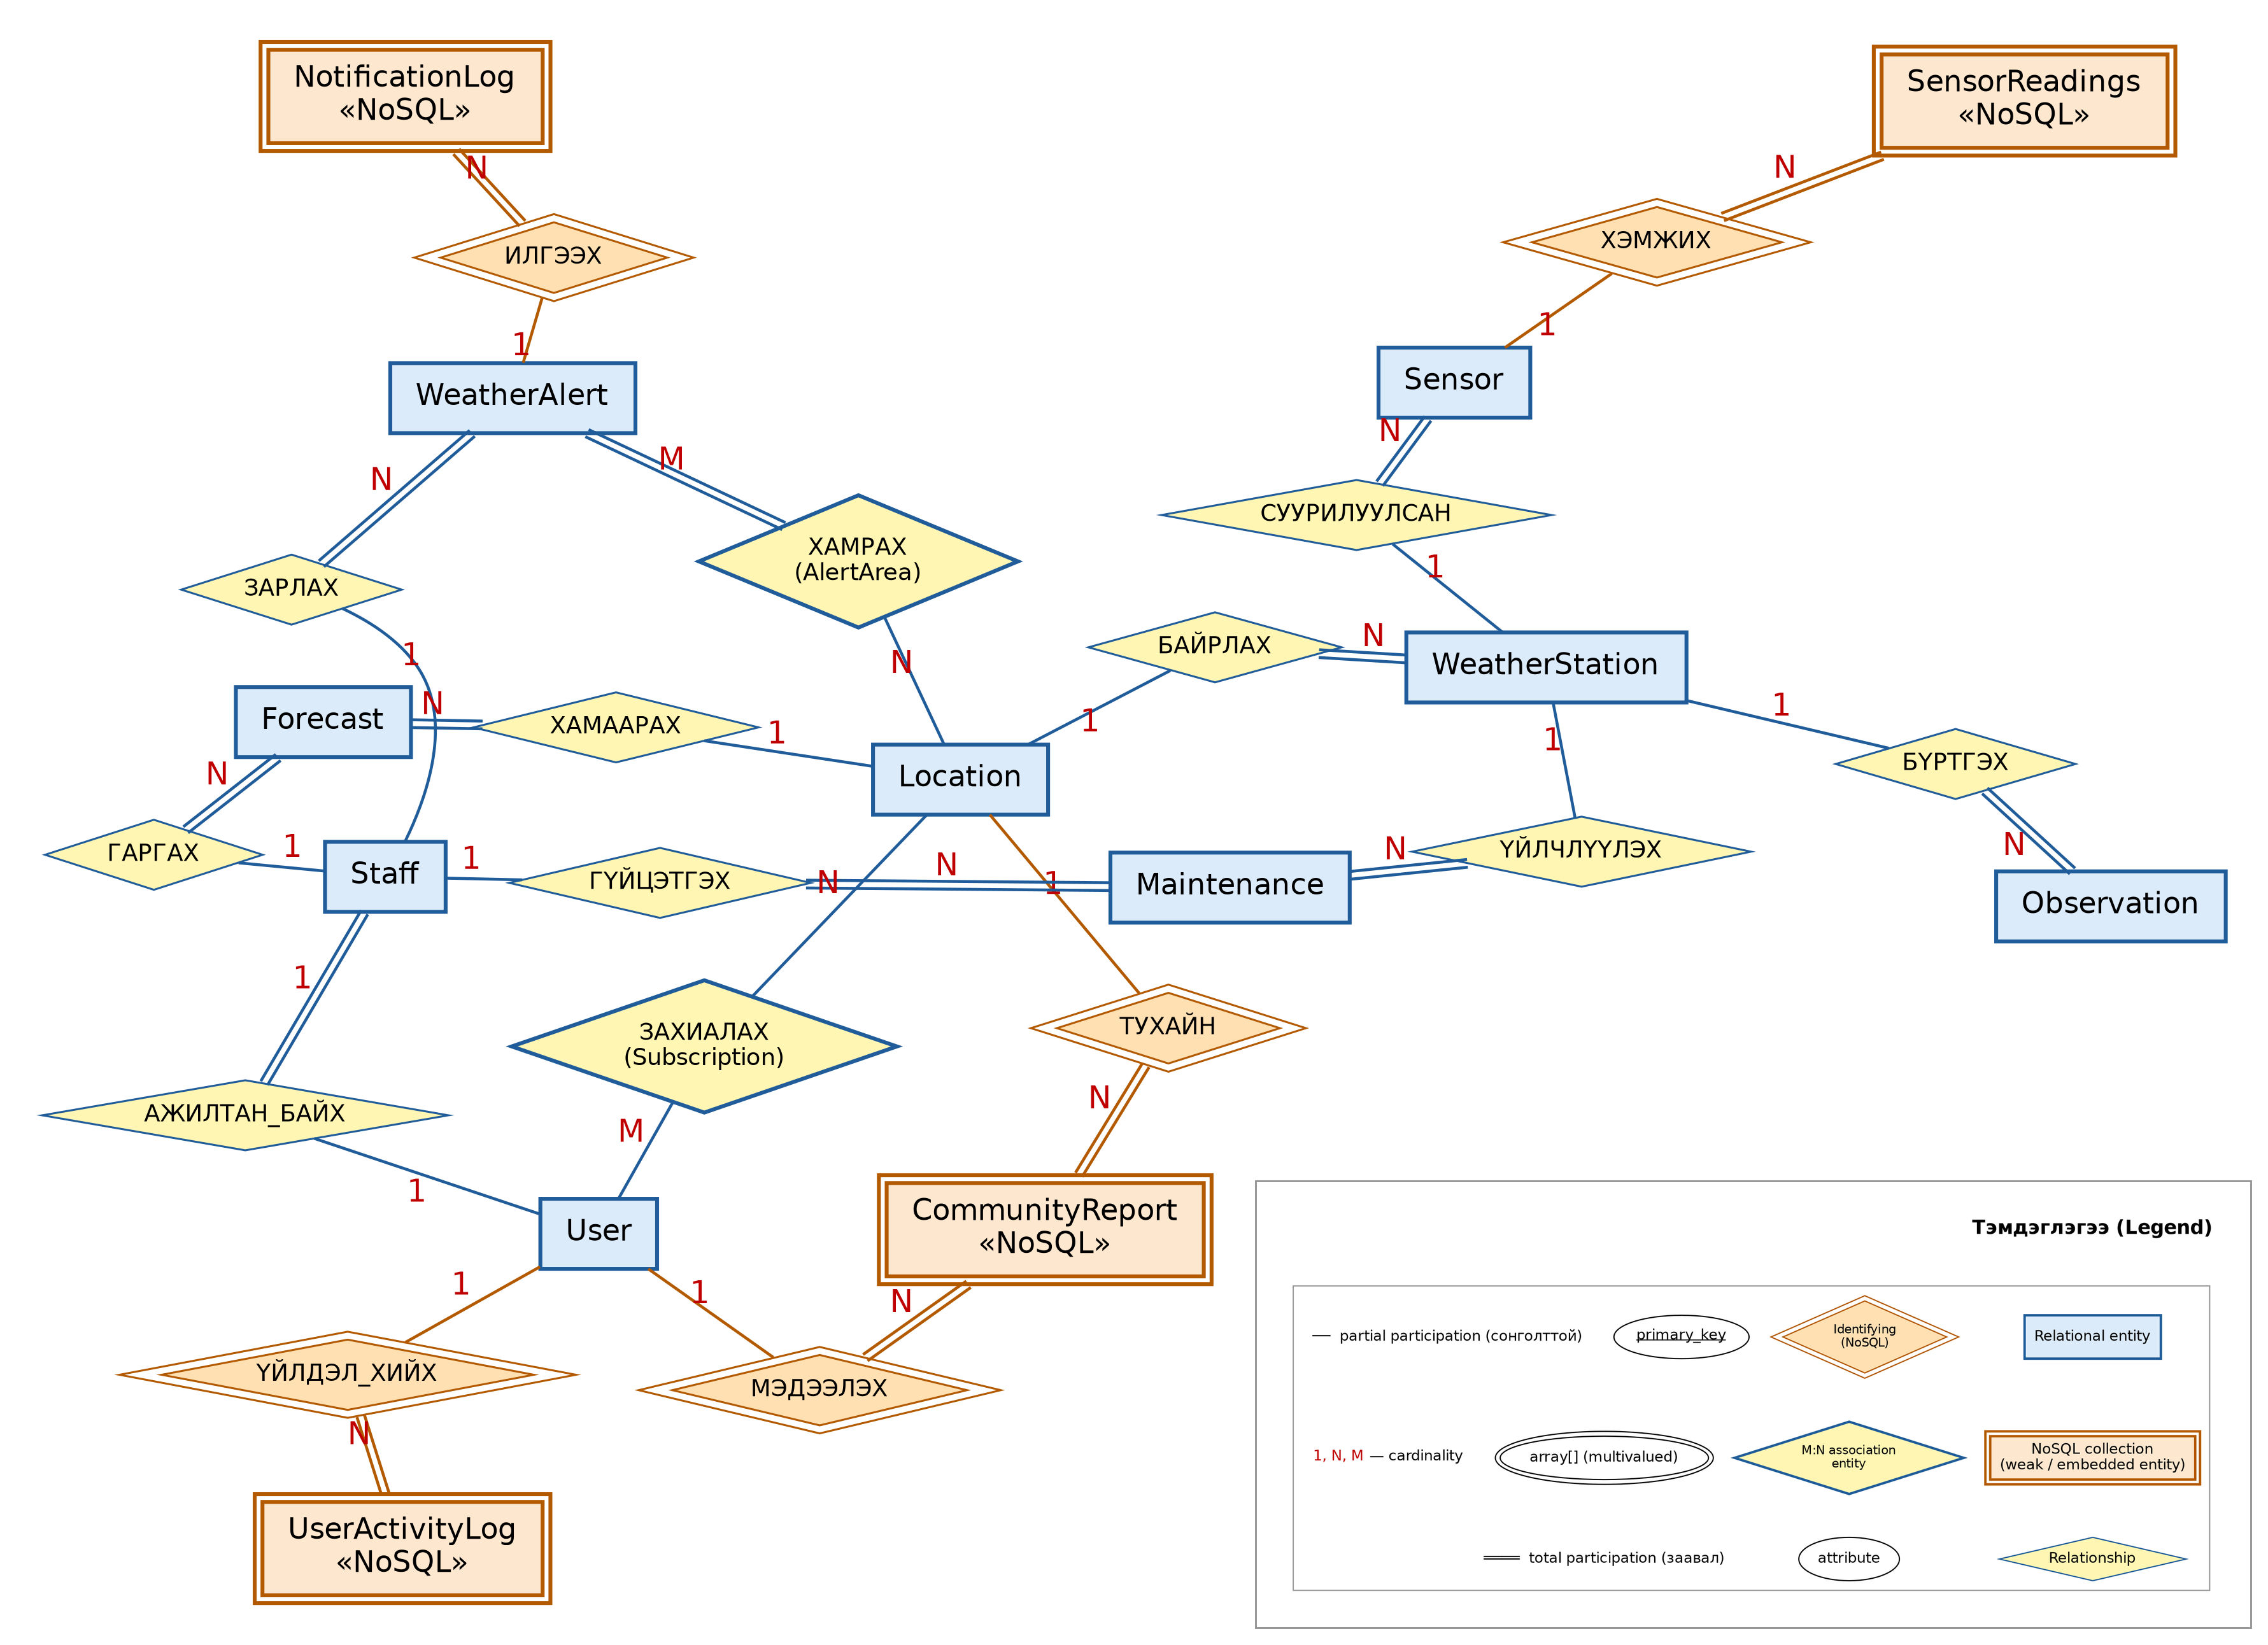
\includegraphics[width=\linewidth,height=0.93\textheight,keepaspectratio]{images/erd_overview.png}
\caption{Ерөнхий Chen ERD: entity, холбоос, cardinality ба participation}\label{fig:erd}
\end{figure}
\begin{figure}[p]
\centering
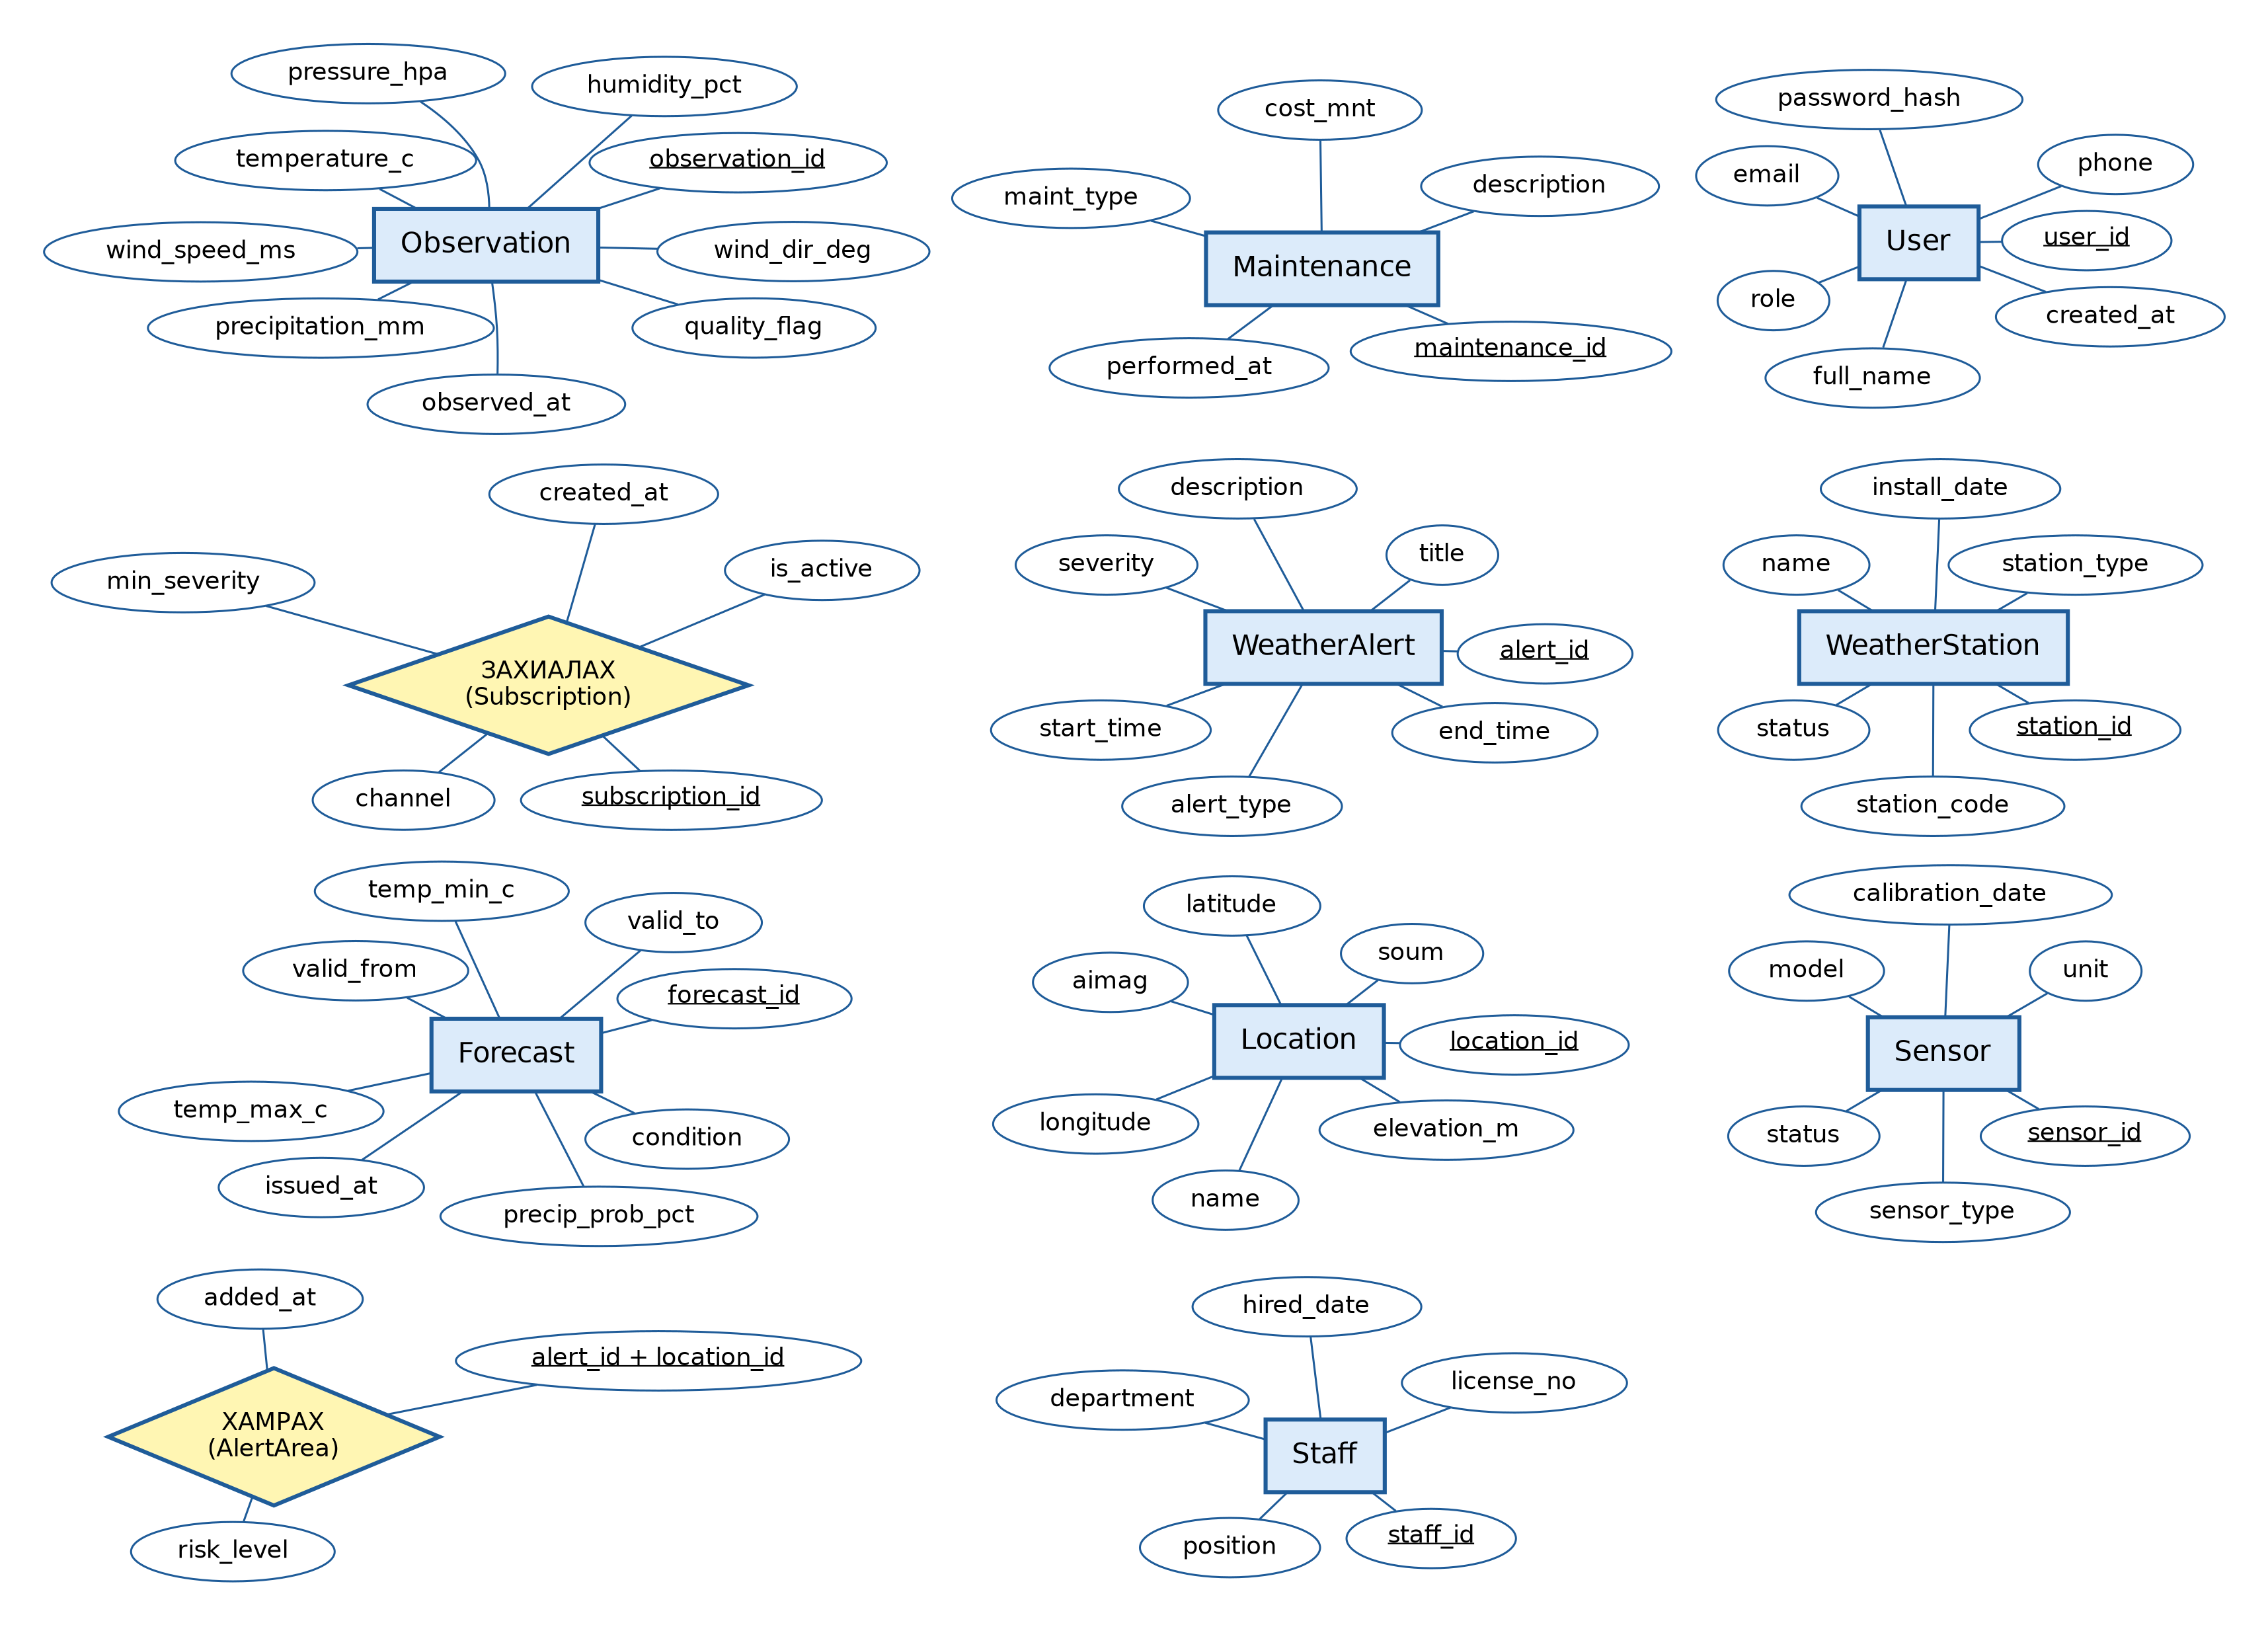
\includegraphics[width=\linewidth,height=0.93\textheight,keepaspectratio]{images/erd_rel_attrs.png}
\caption{Relational entity-үүдийн атрибутууд (Chen)}\label{fig:relattr}
\end{figure}
\end{landscape}

\begin{figure}[htbp]
\centering
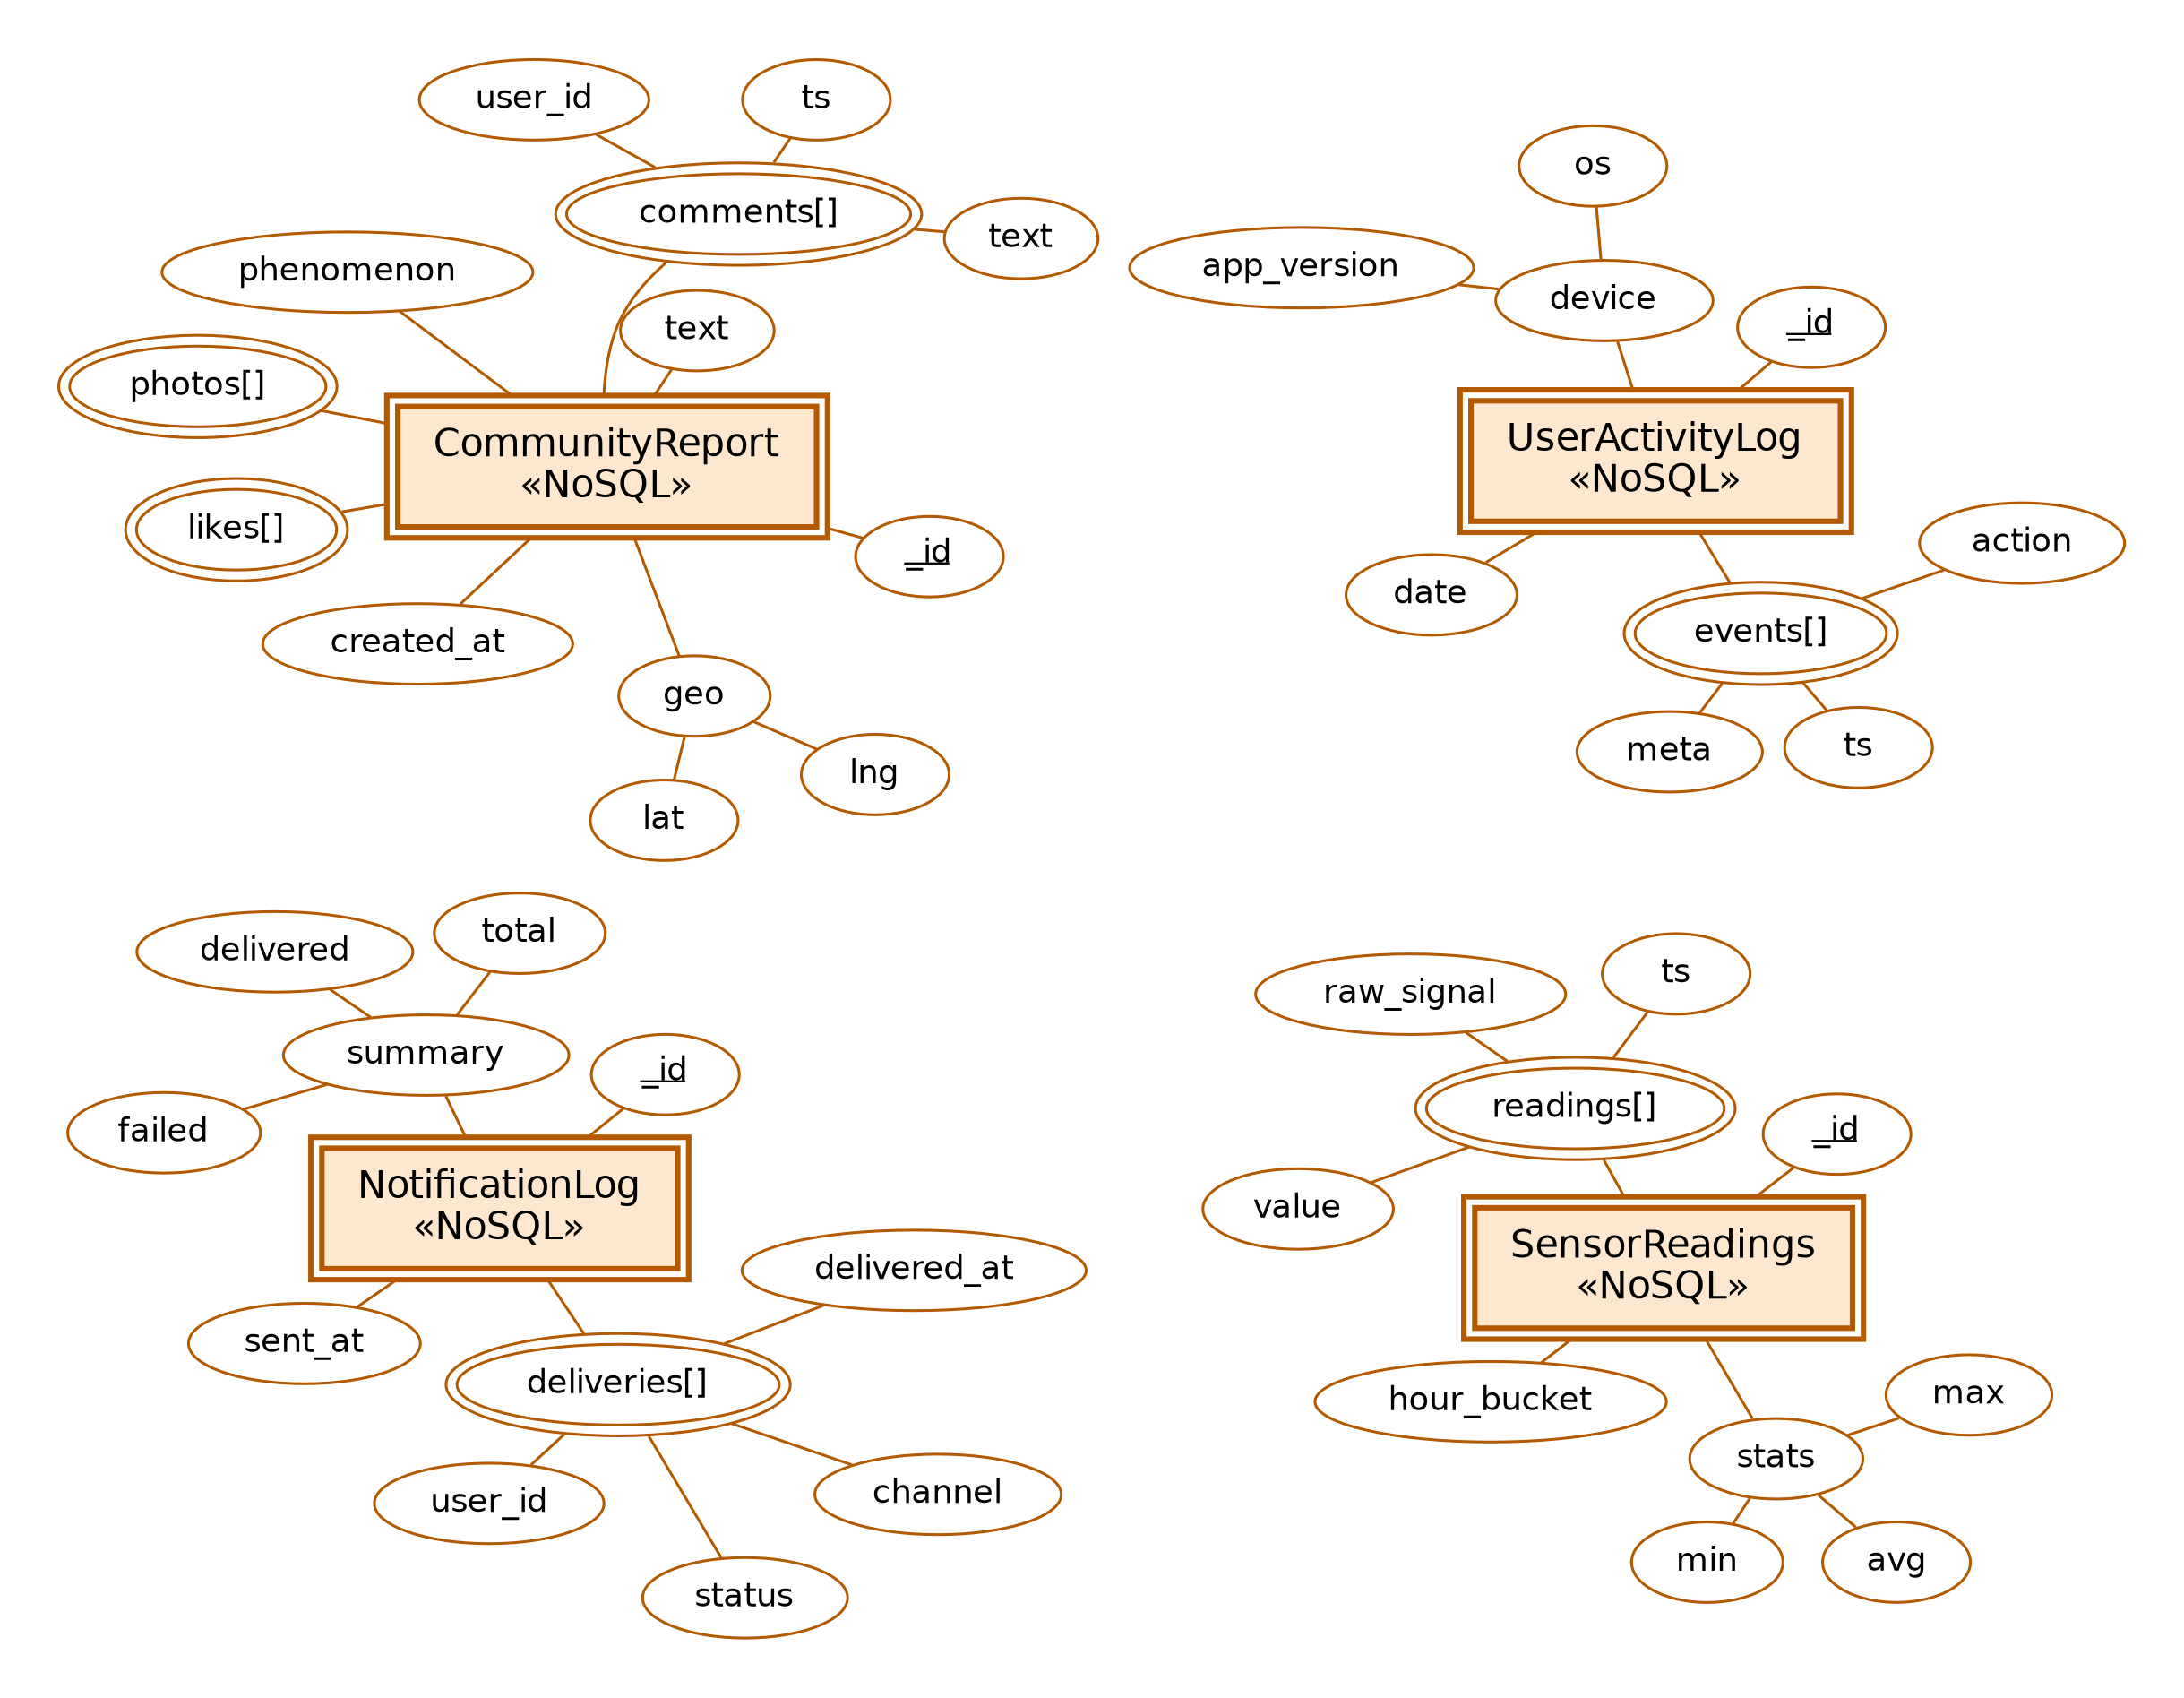
\includegraphics[width=\textwidth]{images/erd_nosql_attrs.png}
\caption{NoSQL collection-уудын атрибут, embedded document ба array (Chen)}\label{fig:nosqlattr}
\end{figure}


% =====================================================================
\section{Relational vs NoSQL шийдлийн тайлбар}
% =====================================================================
Баталгаатай, хоорондоо нягт холбоостой бизнесийн өгөгдлийг
\textbf{relational}, их хэмжээгээр бичигддэг, бүтэц нь хувьсдаг, үргэлж
хамт уншигддаг лог/түүхийг \textbf{NoSQL (document)} хэлбэрээр хадгалах
холимог (polyglot) загвар сонгосон.

\subsection{Яагаад relational вэ?}
\begin{itemize}
  \item \textbf{Бүрэн бүтэн байдал:} Forecast заавал бодит Location ба Staff-тай, Sensor заавал станцтай байх ёстой — FK ба constraint-оор баталгаажна.
  \item \textbf{ACID гүйлгээ:} сэрэмжлүүлэг ба түүний хамрах нутгуудыг (WeatherAlert + AlertArea) нэг гүйлгээгээр хадгалах хэрэгтэй; хагас нь хадгалагдвал иргэдэд буруу сэрэмжлүүлэг очно.
  \item \textbf{M:N холбоос ба JOIN:} «Энэ сэрэмжлүүлгийг аль захиалагчид авах вэ?» гэсэн асуулга WeatherAlert $\rightarrow$ AlertArea $\rightarrow$ Subscription $\rightarrow$ User JOIN-оор шууд хариулагдана.
  \item \textbf{Тогтвортой бүтэц, тайлан:} Observation-ийн баганууд (температур, даралт…) стандарт тул сарын дундаж, аймгийн харьцуулалт зэрэг SQL агрегат тайланд тохиромжтой.
\end{itemize}

\subsection{NoSQL entity бүрийг сонгосон шалтгаан}
{\small
\begin{longtable}{L{2.8cm}L{4.2cm}L{8.0cm}}
\caption{NoSQL collection-уудыг сонгосон үндэслэл}\label{tab:why}\\
\toprule
\textbf{Collection} & \textbf{Загвар} & \textbf{Relational-д яагаад тохиромжгүй вэ}\\
\midrule
\endfirsthead
\toprule
\textbf{Collection} & \textbf{Загвар} & \textbf{Relational-д яагаад тохиромжгүй вэ}\\
\midrule
\endhead
\bottomrule
\endfoot
SensorReadings & Time-series bucket: цаг бүрийн 60 утга \texttt{readings[]} array-д & 500 станц × 6 мэдрэгч × 1440 минут $\approx$ 4.3 сая мөр/өдөр — нэг хүснэгтэд бичвэл index хэт томроно; bucket нь бичилтийг 60 дахин цөөлнө. Мэдрэгчийн төрлөөс хамаарч талбар өөр (raw\_signal, нэмэлт төлөв).\\
UserActivityLog & Өдөр бүрийн баримт, \texttt{events[]} ба embedded \texttt{device} & Зөвхөн нэмэгддэг (append-only), засварлагддаггүй; үйлдэл бүрийн \texttt{meta} талбар өөр бүтэцтэй. JOIN шаарддаггүй, хуучирсан логийг TTL-ээр автоматаар устгана.\\
NotificationLog & Сэрэмжлүүлэг бүрт нэг баримт, \texttt{deliveries[]} ба \texttt{summary} & Нэг сэрэмжлүүлэг зуун мянган хүнд янз бүрийн сувгаар очно; SMS/push үйлчилгээний хариу өөр талбартай. Илгээлтийн түүхийг сэрэмжлүүлэгтэй нь хамт нэг уншилтаар авна.\\
CommunityReport & Мэдээлэл + embedded \texttt{geo}, \texttt{photos[]}, \texttt{comments[]}, \texttt{likes[]} & Нийгмийн сүлжээний пост шиг — сэтгэгдэл, like зэрэг тоо нь тогтмол бус өгөгдөл хэлбэрт үргэлж хамт харагдана. Relational-д 3–4 хүснэгт ба JOIN шаардах байсан. Geo index-ээр «ойролцоох мэдээлэл» хайна.\\
\end{longtable}
}

\subsection{Хоёр хэсгийн холбоос}
\begin{itemize}
  \item NoSQL баримт бүр relational entity-г \textbf{ID-гаар лавлана} (\texttt{sensor\_id}, \texttt{user\_id}, \texttt{alert\_id}, \texttt{location\_id}) — энэ нь ERD дээрх identifying relationship.
  \item Гол урсгал: \texttt{SensorReadings} (NoSQL) $\rightarrow$ цаг бүр нэгтгэж \texttt{Observation} (SQL) $\rightarrow$ \texttt{Forecast} / \texttt{WeatherAlert} (SQL) $\rightarrow$ илгээлт \texttt{NotificationLog} (NoSQL).
  \item NoSQL тал нь eventual consistency-тэй байсан ч болно: лог болон түүхий хэмжилт хэдэн секунд хоцорсноор бизнесийн алдаа гарахгүй.
\end{itemize}

\subsection{Баримтын жишээ (CommunityReport)}
\begin{Verbatim}[fontsize=\small,frame=single,framesep=3mm,samepage=true]
{
  "_id": "rep_20260928_0412",
  "user_id": 1052,
  "location_id": 37,
  "created_at": "2026-09-28T14:20:00+08:00",
  "phenomenon": "мөндөр",
  "text": "Цэцэрлэг суманд 5 минут мөндөр орлоо",
  "geo": { "lat": 47.47, "lng": 101.45 },
  "photos": ["https://cdn.example/r0412_1.jpg"],
  "comments": [
    { "user_id": 2201, "text": "Манайд бас орсон",
      "ts": "2026-09-28T14:31:00+08:00" }
  ],
  "likes": [2201, 3310, 4127]
}
\end{Verbatim}

\clearpage
% =====================================================================
\section*{Дүгнэлт}
\addcontentsline{toc}{section}{Дүгнэлт}
% =====================================================================
Энэхүү лабораторийн ажлаар цаг агаарын мэдээллийн системийн шаардлагыг
тодорхойлж, түүнд тулгуурлан 15 entity бүхий өгөгдлийн сангийн conceptual
загварыг Chen ERD-ээр боловсруулав. Хэрэглэгч, байршил, станц, урьдчилсан
мэдээ, сэрэмжлүүлэг зэрэг бүрэн бүтэн байдал, гүйлгээ шаарддаг 11 entity-г
relational хэлбэрээр загварчилж, 1:1, 1:N болон association entity ашигласан
M:N холбоосуудыг cardinality, participation-ийн хамт тодорхойлов.

Харин минут тутмын мэдрэгчийн хэмжилт, хэрэглэгчийн үйлдлийн лог, мэдэгдэл
илгээлтийн түүх, иргэдийн мэдээлэл зэрэг их хэмжээтэй, бүтэц нь хувьсдаг
4 өгөгдлийг NoSQL document хэлбэрээр embedded document болон array ашиглан
загварчилсан. Ингэснээр гол бизнесийн өгөгдлийн найдвартай байдал болон
их хэмжээний өгөгдлийн уян хатан, хурдан бичилтийг нэг системд хослуулах
холимог (polyglot) шийдэл гарлаа.

% Дүгнэлтийн дараах 1 хоосон хуудас
\clearpage
\thispagestyle{empty}
\mbox{}
\clearpage

\end{document}
